\section{设计思想(本程序中的用到的主要算法及数据结构)}

\subsection{生成数据}

基于$sin(2\pi x)$产生$N$个样本,横轴坐标为

\begin{equation}
    x =
    \begin{bmatrix}
        x_1 \\ x_2 \\ \vdots \\ x_N
    \end{bmatrix}
\end{equation}

对应的纵轴坐标为

\begin{equation}
    y =
    \begin{bmatrix}
        y_1 \\ y_2 \\ \vdots \\ y_N
    \end{bmatrix}
\end{equation}

对其中的每一个$y_i$加上一个$\mu = 0$,$\sigma = 0.1$的高斯噪声,得到新的纵轴数据

\begin{equation}
    T =
    \begin{bmatrix}
        t_1 \\ t_2 \\ \vdots \\ t_N
    \end{bmatrix}
\end{equation}

可得下图

\begin{figure}[H]
    \centering
    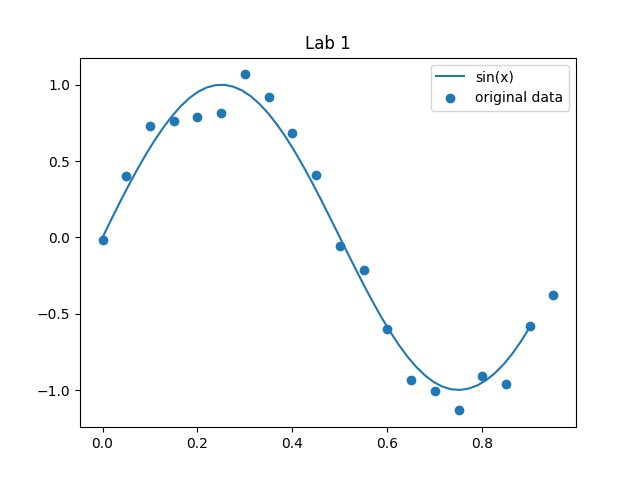
\includegraphics[width=0.7\textwidth]{figures/Figure_1.png}
    \caption{生成原始数据}
\end{figure}

\subsection{多项式拟合}

\subsubsection{误差函数}

根据泰勒展开公式,我们可以用公式\eqref{yxw}所示的多项式函数来尝试拟合一个未知的曲线

\begin{equation}
    y(x, w) = w_0 + w_1 x + \ldots + w_m x^m = \sum_{i = 1}^{m} w_i x^i
    \label{yxw}
\end{equation}

其中$x$前的参数

\begin{equation}
    w = 
    \begin{bmatrix}
        w_0 \\ w_1 \\ \vdots \\ w_m
    \end{bmatrix}
\end{equation}

是我们想要求的

根据最小二乘法,误差函数为

\begin{equation}
    E(w) = \frac{1}{2} \sum_{n=1}^{N} \{ y(x_n, w) - t_n \}^2
    \label{loss}
\end{equation}

只需最小化此误差函数

我们有如下三种方案

\subsection{误差函数最小化}

\subsubsection{解析解法}

解析解推导过程如下:

设

\begin{equation}
    x_n =
    \begin{bmatrix}
        x_n^0 \\ x_n^1 \\ \ldots \\ x_n^m
    \end{bmatrix}
\end{equation}

以及

\begin{equation}
    X =
    \begin{bmatrix}
        x_1^T \\ x_2^T \\ \ldots \\ x_N^T
    \end{bmatrix}
\end{equation}

可得

\begin{equation}
    y(x_n, w) = x_n^T \cdot w
\end{equation}

则

\begin{align}
    2 E(w)  &= \sum_{n=1}^{N} \{ y(x_n, w) - t_n \}^2 \\
            &=  \begin{bmatrix}
                    y_1(x_1, w) - t_1 \\ \vdots \\ y_N(x_N, w) - t_N
                \end{bmatrix}
                ^T
                \cdot 
                \begin{bmatrix}
                    y_1(x_1, w) - t_1 \\ \vdots \\ y_N(x_N, w) - t_N
                \end{bmatrix} \\
            &=  \begin{bmatrix}
                    x_1^T w - t_1 \\ \vdots \\ x_N^T w - t_N
                \end{bmatrix}
                ^T
                \cdot 
                \begin{bmatrix}
                    x_1^T w - t_1 \\ \vdots \\ x_N^T w - t_N
                \end{bmatrix} \\
            &=  \left(
                \begin{bmatrix}
                    x_1^T \\ \vdots \\ x_N^T    
                \end{bmatrix}
                \cdot
                w - T
                \right)^T
                \cdot
                \left(
                \begin{bmatrix}
                    x_1^T \\ \vdots \\ x_N^T    
                \end{bmatrix}
                \cdot
                w - T
                \right) \\
            &=  \left(
                    X w - T
                \right)^T
                \cdot
                \left(
                    X w - T
                \right) \\
            &=  \left(
                    w^T X^T - T^T
                \right)
                \cdot
                \left(
                    X w - T
                \right) \\
            &=  w^T X^T X w - w^T X^T T - T^T X w + T^T T \\
            &=  w^T X^T X w - 2 w^T X^T T + T^T T
\end{align}

对$w$求导,可得

\begin{equation}
    \frac{\partial E}{\partial w} = \frac{1}{2} \left( 2 X^T X w - 2 X^T T \right)
\end{equation}

令其为$0$,可得线性方程组

\begin{equation}
    X^T X w = X^T T
    \label{linear-equ}
\end{equation}

方程\eqref{linear-equ}的解为

\begin{equation}
    w = \left( X^T T \right)^{-1} X^T T
\end{equation}

注意到其中的$X^T X$是半正定的,不一定可逆。当$X^T X$不可逆时,可以用

\begin{equation}
    w = \left( X^T T + \epsilon E \right)^{-1} X^T T
\end{equation}

作为$w$的解,其中$\epsilon$是足够小的正数

使用Numpy求出解析解的代码如下

\rule{\textwidth}{0.01em}
\begin{verbatim}
    # 生成矩阵 X 及其转置 XT
    XT = []
    for i in range(0, m + 1):
        for j in range(0, N):
            XT.append(x[j] ** i)
    XT = np.reshape(XT, (m + 1, N))
    X = np.transpose(np.array(XT))

    # 解析解: (XT * X + lambda * E) * w = XT * T
    w = np.dot(
        np.linalg.inv(
            np.dot(XT, X) + lam * np.identity(m + 1)
        ),
        np.dot(XT, T)
    )
\end{verbatim}
\rule{\textwidth}{0.01em}

\subsubsection{梯度下降法}

梯度下降法可以找到一个函数的局部极小值,由于在拟合曲线问题中,$E(w)$是关于$w$的二次函数,所以找到的极小值就是我们期望的最小值

梯度下降法的迭代公式如下

\begin{equation}
    w = w - \alpha \frac{\partial E(w)}{\partial w}
\end{equation}

其中$\alpha$为学习率,相当于梯度下降时每一步的步长。此学习率不宜过大

使用Numpy运行梯度下降法算法的代码如下

\rule{\textwidth}{0.01em}
\begin{verbatim}
    # 梯度下降
    alpha = 0.01  # 学习率
    turn = 10000  # 迭代次数
    w = np.ones(m + 1)
    for i in range(0, turn):
    w = w - alpha * (
        np.dot(np.dot(XT, X), w)
        - np.dot(XT, T)
        + lam * np.dot(np.identity(m + 1), w)
    )
\end{verbatim}
\rule{\textwidth}{0.01em}

\subsubsection{共轭梯度法}

对使用解析解求解线性方程组时,于计算机而言求矩阵的逆非常复杂,计算量甚至和矩阵相乘的计算量相当\cite{ref1}。当矩阵维数非常大时(即数据非常多),矩阵求逆会十分缓慢。此时可以采用共轭梯度法,通过迭代的方式求解线性方程组。

对于求解

\begin{equation}
    A x = b
\end{equation}

使用共轭梯度法伪代码如下\cite{ref2}:

\rule{\textwidth}{0.01em}
\begin{align}
    \notag
    r_0 &=  b - A x_0 \\
    \notag
    p_0 &=  r_0 \\
    \notag
    k   &=  0 \\
    \notag
    LOOP: \\
    \notag
    \alpha_k    &=  \frac{r_k^T r_k}{p_k^T A p_k} \\
    \notag
    x_{k + 1}   &=  x_k + \alpha_k p_k \\
    \notag
    r_{k + 1}   &=  r_k - \alpha_k A p_k \\
    \notag
    if \quad r_{k + 1} < \epsilon \\
    \notag
    break \\
    \notag
    \beta_k     &=  \frac{r_{k + 1}^T r_{k + 1}}{r_k^T r_k} \\
    \notag
    p_{k + 1}   &=  r_{k + 1} + \beta_k p_k \\
    \notag
    k           &=  k + 1 \\
    \notag
    goto \quad LOOP
\end{align}
\rule{\textwidth}{0.01em}

最终结果为$x_{k + 1}$

使用Numpy并将共轭梯度法封装为函数的代码如下

\rule{\textwidth}{0.01em}
\begin{verbatim}
def cgm(A: np.matrix, b: np.array, size: int) -> list:
    """共轭梯度法求线性方程组 Ax = b 的解

    Args:
        A:    size * size 的矩阵
        b:    size * 1    的列向量
        size: 维数,即 b.shape[0]

    Returns:
        返回线性方程组的解 x
    """

    x = np.ones(size)
    r_old = b - np.dot(A, x)
    p = r_old.copy()
    for i in range(0, 10):
        a = np.dot(r_old.T, r_old) / np.dot(np.dot(p.T, A), p)
        x = x + np.dot(a, p)
        r_new = r_old - np.dot(np.dot(a, A), p)
        if np.dot(r_new.T, r_new) < 1e-10:
            break
        bb = np.dot(r_new.T, r_new) / np.dot(r_old.T, r_old)
        p = r_new + np.dot(bb, p)
        r_old = r_new

    return x
\end{verbatim}
\rule{\textwidth}{0.01em}

\subsection{带惩罚项的误差函数}

设误差函数\eqref{loss}的最优解为$w^{\star}$,当阶数$m$较大时,$w_i^{\star}$变化非常剧烈,将导致过拟合等问题。为此,可以在$E(w)$中加入对$w$的惩罚。

修改后的误差函数如下

\begin{equation}
    E(w) = \frac{1}{2} \sum_{n=1}^{N} \{ y(x_n, w) - t_n \}^2 + \frac{\lambda}{2} \left\lVert w \right\rVert ^2
\end{equation}

其中$\left\lVert w \right\rVert ^2$是$w$的二范数,即

\begin{equation}
    \left\lVert w \right\rVert ^2 = w^T w = w_1^2 + \ldots + w_m^2
\end{equation}

加入此正则项后,通过相似的推导,可得最小二乘法最终的线性方程组,即

\begin{equation}
    \left( X^T X + \lambda E \right) w = X^T T    
\end{equation}

通过对函数的封装,可以正常使用解析解法、梯度下降法、共轭梯度法求出改良后的$w^{\star}$
